\documentclass{article}
\usepackage[utf8]{inputenc}
\usepackage[english]{babel}
\usepackage{amsmath}
\usepackage[]{amsthm}
\usepackage[]{amssymb} 
\usepackage{mathrsfs}
\usepackage{tcolorbox}
\usepackage{nicefrac}
\usepackage{mathtools}
% \usepackage{graphicx}
\usepackage{caption}
\usepackage{subcaption}
\usepackage{tikz}
\usepackage{tabularx}
\usepackage{array}

% \graphicspath{ {./images/} }

\theoremstyle{definition}
\newtheorem*{claim}{Claim}
\newtheorem*{corollary}{Corollary}
\DeclareMathOperator{\adj}{\operatorname{adj}}
\DeclareMathOperator{\im}{\operatorname{im}}
\DeclareMathOperator{\spn}{\operatorname{span}}
\DeclareMathOperator{\nll}{\operatorname{null}}
\newcommand{\R}{\mathbb{R}}
\newcommand{\Z}{\mathbb{Z}}
\newcommand{\N}{\mathbb{N}}
\newcommand{\F}{\mathbb{F}}
\newcommand{\C}{\mathbb{C}}
\newcommand{\D}{\operatorname{D}}
\newcommand{\GL}{\operatorname{GL}}
\newcommand{\SL}{\operatorname{SL}}
\newcommand{\GLnR}{\GL_n(\R)}
\newcommand{\SLnR}{\SL_n(\R)}
\newcommand{\trace}{\operatorname{tr}}
\DeclarePairedDelimiter\floor{\lfloor}{\rfloor}
\DeclarePairedDelimiter\set{\{}{\}}
\DeclarePairedDelimiter\abs{\lvert}{\rvert}
\DeclarePairedDelimiter\genby{\langle}{\rangle}
\newcommand{\restrict}[1]{ \big|_{#1} }


\title{18.701: Problem Set 6}
\author{Dmitry Kaysin}
\date{April 2020}
\begin{document}
\maketitle 


\subsection*{Preliminary Problem 1}

\begin{tcolorbox}
Let $\ell_1$ and $\ell_2$ be lines through the origin in $\R^2$ that intersect in an angle $\pi / n$, and let $r_i$ be the reflection about $\ell_i$.
Prove that $r_1$ and $r_2$ generate a dihedral group $\D_n$.
\end{tcolorbox}

\begin{proof}

Denote $\theta$ the oriented angle between $\ell_1$ and $\ell_2$.
Since $r_1$ and $r_2$ are isometries, they must generate a group of symmetries of the plane $\R^2$, denote it $G$.
Choose coordinates in such a way that $r_1$ is a reflection about $e_1$.
Then $r_2 = \rho_\theta r_1 \rho_{-\theta}$, and $r_2 r_1$ is rotation around the origin by angle $2\theta$:
\[
    \rho_\theta r_1 \rho_{-\theta} r_1
    = \rho_\theta r_1 r_1 \rho_{\theta}
    = \rho_{2\theta}.
\]
Denote $r_2 r_1 = \rho_{2\theta}$ as $\rho$ for the sake of simplicity.

We can see that $\rho^n$ is a rotation around the origin by angle $2\pi$, hence $\rho^n = 1$.
Subgroup $\genby{\rho}$ is cyclic, thus each power of $\rho$ has order of at most $n$.
Inverse rotation $\rho^{-1}$ is equivalent to $\rho^{n-1}$.

Consider homomorphism $\varphi : G \to \set{-1,1}$, which maps plane isometry to the sign of the determinant of the matrix that represents such isometry in arbitrary coordinates.
Thus, $\varphi$ separates orientation-preserving and orientation-reversing isometries.
Subgroup $\genby{\rho}$ is the kernel of $\varphi$, thus a normal subgroup.
Since $\genby{\rho}$ is normal, its left and right cosets are the same. 
Consider coset $\genby{\rho} r_1$:
any of its elements is distinct from elements of $\genby{\rho}$, which can be confirmed by examining their respective matrix representations.
We note that $r_2 = \rho r_1^{-1} = \rho r_1$ is in this coset.
Therefore $G$ consists of subgroup $\genby{\rho}$ and its single coset $\genby{\rho} r_1$:
\[
    G = \set{
        1, \> \rho, \> \rho^2, \> \dots, \> \rho^{n-1}, \>
        r_1, \> \rho r_1, \> \rho^2 r_1, \> \dots, \> \rho^{n-1} r_1.
    }
\]

From this we conclude that $G$ is finite and has order $2n$.
It is easy to see that every element of $G$ is an orthogonal operator.
Finite group of orthogonal operators on the plane is either a cyclic group or a dihedral group.

Cyclic group of order $2n$ must have an element of order $2n$.
However, the maximum order of the element of $G$ is $n$.
Therefore $G$ is a dihedral group $D_n$ of order $2n$.

\end{proof}


\subsection*{Preliminary Problem 2}

\begin{tcolorbox}
Let $(a,b)$ be a lattice basis of a lattice $L$ in $\R^2$.
Prove that every other lattice basis has the form $(a',b') = (a,b)P$, where $P$ is a $2 \times 2$ integer matrix with determinant $\pm 1$.
\end{tcolorbox}

\begin{proof}

Let $B' = (a',b')$ be an arbitrary basis of $L$.
It can be written in terms of the basis $B=(a,b)$:
\begin{gather*}
    a' = m_1 a + n_1 b, \\
    b' = m_2 a + n_2 b,
    \shortintertext{or}
    B' =
    B P,
    \shortintertext{where}
    P =
    \begin{pmatrix}
        m_1 & m_2 \\
        n_1 & n_2
    \end{pmatrix}
\end{gather*}
is a $2 \times 2$ matrix with integer entries.

Consider arbitrary vector $V \in L$.
It can be written in terms of the basis $B$:
\begin{gather*}
    V = B X,
    \shortintertext{where}
    X =
    \begin{pmatrix}
        m \\
        n
    \end{pmatrix}
\end{gather*}
is a vector with integer entries.

Coordinates of $V$ in the basis $B'$ are $P^{-1}X$, hence $P^{-1}$ must have integer entries.
As we have seen in Artin, Chapter 1, Exercise 6.2, matrix with integer entries is invertible and its inverse has integer entries, if and only if its determinant is $\pm 1$.
This proves the needed assertion.

\end{proof}


\subsection*{Problem 1}

\begin{tcolorbox}
Let $N'$ be the group of isometries of an infinite ribbon
\[ R = \set{(x,y) : -1 \leq y \leq 1}. \]
The following elements are in $N'$:
\begin{align*}
    t_a : (x,y) & \longmapsto (x+a,y), \\
    s : (x,y) & \longmapsto (-x,y), \\
    r : (x,y) & \longmapsto (x,-y), \\
    \rho : (x,y) & \longmapsto (-x,-y).
\end{align*}

A frieze pattern is a pattern on the ribbon that is periodic and whose group of symmetries is discrete.
Classify the corresponding symmetry groups, identifying those that differ in the choice of origin and unit length on the ribbon.
\end{tcolorbox}

We notice the following relations between elements of $N'$:
\begin{gather*}
    s^2 = r^2 = \rho^2 = 1, \quad
    s r = rs = \rho, \quad
    s \rho = \rho s = r, \quad
    r \rho = \rho r = s, \\
    s t_a = t_{-a} s, \quad
    r t_a = t_a r, \quad
    \rho t_a = t_{-a} \rho.
\end{gather*}

Translation group $L$ of $G$ is discrete and after appropriate scaling becomes $\Z (1,0)$ with basis $(1,0)$.

\begin{claim}
$\overline{N'}$ is a dihedral group $\D_2$
\end{claim}

\begin{proof}
Since $N'$ is discrete, its point group $\overline{N'} = \pi (N')$ is also discrete, thus $\overline{N'}$ must be either a cyclic group or a dihedral group.
By examining the relations, we can see that
\[ \overline{N'} = \set{1, \overline{s}, \overline{r}, \overline{\rho}}, \]
and order of each element of $\overline{N'}$ other than identity is $2$.
Since order of $\overline{N'}$ is $4$, it cannot be a cyclic group.
Therefore $\overline{N'}$ is a dihedral group $\D_2$.
\end{proof}

Using a geometric argument, we note that reflection about a horizontal line in $G$ must be a reflection about the line $y=0$.
We also note that if $G$ contains some reflection about vertical line $\ell$, then it also contains reflection about line $\ell + (1/2,0)$ shifted by $t_1$:
\[ t_{1/2} s t_{-1/2} = t_1 s. \]
The same is true for a $180^\circ$ rotation in $G$:
\[ t_{1/2} \rho t_{-1/2} = t_1 \rho. \]

Group $G$ of symmetries of a frieze pattern has point group that is a subgroup of $\overline{N'}$.
Possible subgroups of $\overline{N'}$ are:
\[
    \set{1, \overline{r}}, \quad
    \set{1, \overline{s}}, \quad
    \set{1, \overline{\rho}}, \quad
    \set{1, \overline{r}, \overline{s}, \overline{\rho}}.
\]
We proceed to classify possible groups $G$ for each possible subgroup of $\overline{N'}$.

\paragraph{Case 1: $\overline{G} = \set{1}$.}
$G$ is generated by $\set{t_1}$ and is isomorphic to infinite cyclic group $\Z$

\begin{proof}
Point group of $G$ is trivial, thus $G$ contains only translations.
The group of translations is generated by a single element $t_1$, thus $G$ is isomorphic to infinite cyclic group $\Z$.
\end{proof}

\paragraph{Case 2: $\overline{G} = \set{1, \overline{r}}$.}

Since point group of $G$ contains $\overline{r}$, $G$ must contain element $t_v r$ for some $v \in \R$.
Then $(t_v r)^2$ must also be in $G$:
\[ (t_v r)^2 = t_v r t_v r = t_{2v}, \]
which means $(2v,0) \in L$.
This implies that $2v$ must be an integer, which is the case only if $v \in \Z$ or $v \in \Z + \frac{1}{2}$.

\subparagraph{Subcase 2.1: $v \in \Z$.}
$G$ is generated by $\set{t_1, r}$ and is isomorphic to product group $R \times T$, where $R = \genby{r}$ and $T = \genby{t_1}$, the subgroup of translations.
We note that $R \simeq \Z_2$ and $T \simeq \Z$.

\begin{proof}

If $v$ is integer, then $t_v$ is in $G$ and $t_{-v} t_v r = r$ is also in $G$.
The result follows by Artin, Proposition 2.11.4d.
We verify the necessary conditions:

\begin{enumerate}

    \item First, we notice that any element of $G$ can be written as $t_1^n r^k : n \in \Z, \> k \in \set{0,1}$.
    This follows from the First Isomorphism Theorem, which implies that $\overline{G}$ is isomorphic to quotient group $G/T$, hence any element of $G$ is either in $T$ or in its coset $Tr$.
    Therefore $\set{t_1,r}$ generate $G$ and $TR = G$.
    
    \item $R$ is normal since for arbitrary $t_1^n r^k \in G$:
    \[
        (t_1^n r^k)^{-1} r (t_1^n r^k) 
        = r^k t_1^{-n} r t_1^{n} r^k
        = r^{2k+1},
    \]
    which is still an element of $R$.
    $T$ is normal since it is a kernel of homomorphism $\pi$.
    
    \item Intersection of $T$ and $R$ is trivial subgroup $\set{1}$.

\end{enumerate}

\end{proof}

\subparagraph{Subcase 2.2: $v \in \Z + \frac{1}{2}$.}
$G$ is generated by $t_{1/2}r$ and is isomorphic to infinite cyclic group $\Z$.

\begin{proof}

Denote $m = v - \frac{1}{2}$.
Since $t_v r$ is in $G$, $t_{-m} t_v r = t_{1/2} r$ must also be in $G$.
Denote $g = t_{1/2} r$.
We first notice that $r$ is not an element of $G$, otherwise $(g r)r = t_{1/2}$ would be an element of $G$, which is not the case.

We also notice that $g^2 = t_1$, therefore any translation $t_n$ in $G$ can be represented as $g^{2n}$.
We conclude that a single element $g = t_{1/2} r$ generates $G$, therefore $G$ is isomorphic to infinite cyclic group $\Z$.

\end{proof}

\paragraph{Case 3: $\overline{G} = \set{1, \overline{s}}$.}
$G$ is generated by $\set{t_1, s}$.

\begin{proof}

Point group of $G$ contains $\overline{s}$.
If we were to consider the preimage of $\overline{s}$ in the group of isometries of $\R^2$, it would be a glide reflection.
After choosing suitable coordinates, it would have the form $t_u s$ with $u \in L$ being a vector orthogonal to the axis of reflection $s$.
Since we restrict our analysis to a ribbon in $\R^2$, the preimage of $\overline{S}$ in $G$ can only be a reflection about a vertical line.
We choose coordinates so that axis of reflection is the vertical line through the origin, then $G$ contains $s$.

By the First Isomorphism Theorem, every element of $G$ is either in $T$ or in $Ts$, which implies that it has form $t_1^n s^k, n \in \Z, \> k \in \set{0,1}$.
Therefore $\set{t_1, s}$ generate $G$.

\end{proof}

\paragraph{Case 4: $\overline{G} = \set{1, \overline{\rho}}$.}
$G$ is generated by $\set{t_1, \rho}$.

\begin{proof}

Preimage of $\overline{\rho}$ in $G$ can only be a $180^\circ$ rotation about a point on a line $y=0$.
We choose coordinates so that rotation is around the origin, then $G$ contains $\rho$.

Analogous to the previous cases, every element of $G$ has the form $t_1^n \rho^k, n \in \Z, \> k \in \set{0,1}$.
Therefore $\set{t_1, \rho}$ generate $G$.

\end{proof}

\paragraph{Case 5: $\overline{G} = \set{1, \overline{r}, \overline{s}, \overline{\rho}}$.}

By the First Isomorphism Theorem, $G$ consists of normal subgroup $T$, which is the kernel of homomrphism $\pi$, and its three cosets with images $\overline{r}, \overline{s}, \overline{\rho}$, respectively.
We choose coordinates so that $s$ is in $G$.
$G$ must include $t_v \rho$ for some $v \in \R$.
Based on Case 2, $G$ must also include either $r$ or $t_{1/2}r$.

\subparagraph{Subcase 5.1: $G$ includes $r$.}
$G$ is generated by $\set{t_1,r,s}$ and is isomorphic to product group $R \times \genby{t_1, s}$.
We note that $R \simeq \Z_2$.

\begin{proof}

We notice that $t_v \rho r s = t_v$ must be an element of $G$, hence $v \in \Z$.
Then $\rho$ is in $G$.
Therefore any element of $G$ belongs to one of cosets $T$, $Tr$, $Ts$ or $T\rho$.
We know that $rs = \rho$.
Therefore $\set{t_1, r, s}$ generate $G$.

Denote $D = \genby{t_1, s}$.
To prove that $G \simeq R \times D$ we check the conditions of Artin, Proposition 2.11.4d:

\begin{enumerate}

    \item $RD = G$ since generators of $R$ and $D$ together generate $G$.
    \item $R$ is normal since it commutes with all elements of $G$.
    We check that $D$ is normal:
    \begin{gather*}
        (t_a r^b s^c)^{-1} (t_n s^k) (t_a r^b s^c) 
       = s^c r^b t_{-a} t_n s^k t_a r^b s^c
       = s^c r^b t_{n-2a} s^k r^b s^c \\
       = t_{2a-n} s^k r^2b s^2c
       = t_{2a-n} s^k
    \end{gather*}
    \item $R \cap D = \set{1}$.
    
\end{enumerate}

\end{proof}

\subparagraph{Subcase 5.2: $G$ includes $t_{1/2} r$.}
$G$ is generated by $\set{g, s}$ where $g = t_{1/2}r$.

\begin{proof}

We notice that $t_v \rho t_{1/2} r s = t_{v-1/2}$ must be an element of $G$, thus $v - \frac{1}{2}$ must be an integer, hence $v \in \Z + \frac{1}{2}$.
Then $t_{1/2} \rho$ is in $G$.
Therefore $G$ consists of $T$ and its three cosets $T t_{1/2} r$, $Ts$ and $T t_{1/2} \rho$.

We know that $(t_{1/2} r)^2 = t_1$ and $t_{1/2}rs = t_{1/2}\rho$.
Therefore $\set{t_{1/2}r, s}$ generate $G$.

\end{proof}

We note that groups $\genby{t_1, s}, \genby{t_1, \rho}, \genby{t_{1/2}r, s}$ (cases 3, 4, 5.2) are isomorphic.

We present the groups we have identified in the table below (with possible points of origin marked in red). \\
\\
\begin{tabularx} {\textwidth}
    { 
        c
        c
        c
        >{\centering\arraybackslash}X
        c
    }
    &
    Frieze pattern &
    $\overline{G}$ &
    Generators of $G$ &
    $G$
    \\
    &
    \begin{tikzpicture}[baseline=0]
    \path (0, 0) -- (3, 0);
    \draw
        (0, 0) -- (1, 0)
        (0, -0.1) -- (0, 0.1)
        (1, -0.1) -- (1, 0.1)
        (1.2,0) node {$1$};
    \end{tikzpicture}
    \\\\
    % 1
    1 &
    \begin{tikzpicture}[baseline=0]
    \draw (0, 0) -- (3, 0);
    \foreach \x in {0,1,2} {
        \draw 
            ({\x+0.5}, 0) 
            -- ({\x+0.5}, 0.5) 
            -- ({\x}, 0.5);
    }
    \end{tikzpicture}
    & $\set{1}$
    & $\set{t_1}$
    & $\Z$
    \\\\
    % 2.1
    2.1 &
    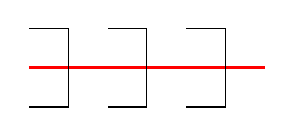
\begin{tikzpicture}[baseline=0]
    \draw[red, thick] (0, 0) -- (3, 0);
    % \draw (0, 0) -- (3, 0);
    \foreach \x in {0,1,2} {
        \draw 
            ({\x+0.5}, 0) 
            -- ({\x+0.5}, 0.5) 
            -- ({\x}, 0.5);
        \draw 
            ({\x+0.5}, 0) 
            -- ({\x+0.5}, -0.5) 
            -- ({\x}, -0.5);
    }
    \end{tikzpicture}
    & $\set{1, r}$
    & $\set{t_1, r}$
    & $\Z_2 \times \Z$
    \\\\
    % 2.2
    2.2 &
    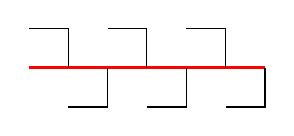
\begin{tikzpicture}[baseline=0]
    \draw[red, thick] (0, 0) -- (3, 0);
    % \draw (0, 0) -- (3, 0);
    \foreach \x in {0,1,2} {
        \draw
            ({\x+0.5}, 0) 
            -- ({\x+0.5}, 0.5)
            -- ({\x+0}, 0.5);
        \draw
            ({\x+1}, 0) 
            -- ({\x+1}, -0.5)
            -- ({\x+0.5}, -0.5);
    }
    \end{tikzpicture}
    & $\set{1, r}$
    & $\set{t_{1/2} r}$
    & $\Z$
    \\\\
    % 3
    3 &
    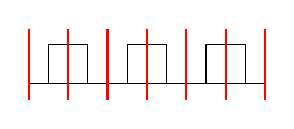
\begin{tikzpicture}[baseline=0]
    \draw (0, 0) -- (3, 0);
    \draw[red, thick] (0, 0.7) -- (0, -0.2);
    \foreach \x in {0,1,2} {
        \draw
            ({\x+0.25}, 0)
            -- ({\x+0.25}, 0.5)
            -- ({\x+0.75}, 0.5)
            -- ({\x+0.75}, 0);
        \draw[red, thick] ({\x+0.5}, 0.7) -- ({\x+0.5}, -0.2);
        \draw[red, thick] ({\x+1}, 0.7) -- ({\x+1}, -0.2);
    }
    \end{tikzpicture}
    & $\set{1, s}$
    & $\set{t_1, s}$ with origin on the lines $x=\frac{1}{2}n, \> n \in Z$
    & $\genby{t_1, s}$
    \\\\
    % 4
    4 &
    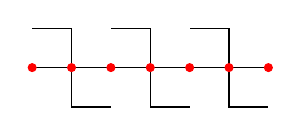
\begin{tikzpicture}[baseline=0]
    \draw (0, 0) -- (3, 0);
    \filldraw[fill=red, draw=red](0,0) circle (0.05);
    \foreach \x in {0,1,2} {
        \draw
            ({\x+0.5}, 0)
            -- ({\x+0.5}, 0.5)
            -- ({\x}, 0.5);
        \draw
            ({\x+0.5}, 0) 
            -- ({\x+0.5}, -0.5)
            -- ({\x+1}, -0.5);
        \filldraw[fill=red, draw=red]({\x+0.5},0) circle (0.05);
        \filldraw[fill=red, draw=red]({\x+1},0) circle (0.05);
    }
    \end{tikzpicture}
    & $\set{1, \rho}$
    & $\set{t_1, \rho}$ with origin at $\left( \frac{1}{2}n,0 \right), \> n \in Z$
    & $\genby{t_1, \rho}$
    \\\\
    % 5.1
    5.1 &
    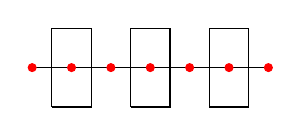
\begin{tikzpicture}[baseline=0]
    \draw (0, 0) -- (3, 0);
    \filldraw[fill=red, draw=red](0,0) circle (0.05);
    \foreach \x in {0,1,2} {
        \draw
            ({\x+0.25}, -0.5) 
            -- ({\x+0.25}, 0.5)
            -- ({\x+0.75}, 0.5)
            -- ({\x+0.75}, -0.5)
            -- ({\x+0.25}, -0.5);
        \filldraw[fill=red, draw=red]({\x+0.5},0) circle (0.05);
        \filldraw[fill=red, draw=red]({\x+1},0) circle (0.05);
    }
    \end{tikzpicture}
    & $\set{1, r, s, \rho}$
    & $\set{t_1, r, s}$ with origin at $\left( \frac{1}{2}n,0 \right), \> n \in Z$
    & $\Z_2 \times \genby{t_1, s}$
    \\\\
    % 5.2
    5.2 &
    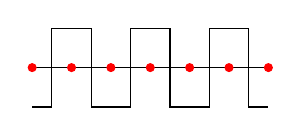
\begin{tikzpicture}[baseline=0]
    \draw (0, 0) -- (3, 0);
    \filldraw[fill=red, draw=red](0,0) circle (0.05);
    \foreach \x in {0,1,2} {
        \draw
            ({\x}, -0.5) 
            -- ({\x+0.25}, -0.5)
            -- ({\x+0.25}, -0.5) 
            -- ({\x+0.25}, 0.5)
            -- ({\x+0.75}, 0.5)
            -- ({\x+0.75}, -0.5)
            -- ({\x+1}, -0.5);
        \filldraw[fill=red, draw=red]({\x+0.5},0) circle (0.05);
        \filldraw[fill=red, draw=red]({\x+1},0) circle (0.05);
    }
    \end{tikzpicture}
    & $\set{1, r, s, \rho}$
    & $\set{t_{1/2}r, s}$ with origin at $\left( \frac{1}{2}n,0 \right), \> n \in Z$
    & $\genby{t_{1/2}r, s}$
\end{tabularx}


\subsection*{Problem 2}

\begin{tcolorbox}
Describe all ways in which $S_3$ can operate on a set of four elements.

Let’s agree to call two operations that differ by a permutation of the set of $4$ equivalent.
I recommend starting your analysis by listing the partitions of a set of $4$.
\end{tcolorbox}

\begin{proof}

Let $A$ and $B$ be sets of $4$ elements.
We say that sets $A$ and $B$ are equivalent ($A \sim B$) if $B$ is a permutation of $A$.

Orbits of the set elements under a group action must partition the set.
We list all possible partitions of the set $A = \set{1,2,3,4}$, unique up to the equivalency relation $\sim$:
\begin{align}
    \set{ \set{1}, \set{2}, \set{3}, \set{4} }, \\
    \set{ \set{1,2}, \set{3}, \set{4} }, \\
    \set{ \set{1,2}, \set{3,4} }, \\
    \set{ \set{1,2,3}, \set{4} }, \\
    \set{ \set{1,2,3,4} },
\end{align}
and examine whether each particular partition of $A$ is possible under $S_3$ acting on $A$.

By the counting formula (Artin 6.9.2), order of each orbit must divide the order of group $G$.
Order of $S_3$ is $6$, thus there is no group action that results in an orbit of order $4$.
Therefore there is no group action of $S_3$ that results in partition (5).

Partition (1) implies that each orbit has order $1$, thus the corresponding group action must be trivial.

Partition (2) implies that the corresponding group action fixes two elements of $A$ (orbits of order $1$), while the other two elements are within an orbit of order $2$.
We notice that the the group $S_2$ acts non-trivially and uniquely on a set of two elements in an obvious way by permuting them.
Denote such group action $m_h, \> h \in S_2$.
If there exists a homomorphism $\varphi : S_3 \to S_2$, then $S_3$ acts on a set of two elements by group action $m_{\varphi(g)}, \> g \in S_3$.
There is indeed such homomorphism, namely the one that maps any permutation to $\pm 1$ according to its sign.
Moreover, there is only one possible homomorphism $S_3 \to S_2$ (which can be seen by the First Isomorphism theorem), hence the corresponding group action is unique.
Since kernel of $\varphi$ is not trivial, action $m_{\varphi(g)}$ is not faithful.
This group action corresponds to the permutation representation $S_3 \to G$, where $G$ is a subgroup of $S_4$ that is generated by any transposition and is isomorphic to $S_2$.

Partition (3) implies two orbits of order $2$ each.
In this case the group action acts by $m_{\varphi(g)}, \> g \in S_3$ (as described above) on each two-element set in the partition.
Again, such group action is unique and is not faithful.
This group action corresponds to the permutation representation $S_3 \to G$, where $G$ is a subgroup of $S_4$ that is generated by two disjoint transpositions and is isomorphic to $S_2$.

Partition (4) implies that the corresponding group action fixes one element of $A$, while the other three elements are within an orbit of order $3$.
Group $S_3$ acts non-trivially on a set of three elements in an obvious way by permuting them.
Such action is faithful since only identity element of $S_3$ leaves all elements of a three-element set fixed.
This group action corresponds to the permutation representation $S_3 \to G$, where $G$ is the subgroup of $G$ isomorphic to $S_3$.

Therefore, there are $3$ possible non-trivial group actions of $S_3$ on the set of $4$ elements.

\end{proof}


\end{document}
